\section{АНАЛИЗ ПРОТОТИПОВ}
\label{sec:solution}

\subsection{Ajenti}
Визитной карточкой панели Ajenti служит приятный интерфейс, реализованный с использованием AJAX. Мы получаем понятную среду, не перегруженную установками и настройками, в которой легко освоится администратор, имеющий относительно небольшой опыт. 

Архитектура модульная, в настоящее время доступны плагины, позволяющие производить настройку и мониторинг самой системы и некоторых популярных сервисов: системных параметров — сети и UPS/питания, пакетных менеджеров, учетных записей пользователей и групп, заданий cron, монтирования дисковых разделов, работы upstart, настройка DNS, правил Netfilter, просмотр журналов; серверов и сервисов — веб (Apache 2, nginx и lighttpd), Samba, MySQL, PostgreSQL, DHCPD, BIND9, NFSD, Squid и SARG, Bacula и других.

В Ajenti нет каких-либо мастеров, которые помогут настроить сервис в пошаговом режиме, поэтому необходимо представлять процесс и параметры. В большинстве случаев плагин предлагает удобную форму для доступа к конфигурационным файлам, частично автоматизируя некоторые операции. Но интерфейс содержит все преднастройки, поэтому часто необходимо лишь заполнить предложенные поля. К тому же новичку будет удобнее править конфиги через браузер, нежели изучать особенности работы с vi. Например, для веб-сервера можно быстро создать виртуальный сайт, буквально одной кнопкой, но заполнять параметры придется самостоятельно.

\subsection{ISPConfig} 
ISPConfig — панель управления хостингом для Linux, которая позволяет настраивать новые веб-сайты, аккаунты электронной почты (POP3, IMAP — Courier, Dovecot), FTP (PureFTPd), записи DNS (BIND, MyDNS), MySQL и виртуализацию OpenVZ. 

При помощи одного интерфейса поддерживается управление несколькими физическими серверами. Обеспечивает настройку виртуального хостинга на основе IP или доменных имен для Apache2 или nginx, работает с PHP через mod\_php, suPHP, fastcgi или PHP-FPM. Поддерживает настройки для FTP, SFTP, SCP и для Apache2 Ruby, Python и WebDAV, реализована проверка на спам (whitelists, blacklists, проверка заголовков и контент-фильтр) и вирусы для входящей почты, email-автоответчик, сбор статистики (Webalizer и/или AWStats), настройка firewall (UFW или bastille), выполнение заданий по расписанию (cron, jailed cron, web cron). Возможно использование shell-доступа для пользователей (обычный и jail), SFTP, SCP, авторизация по паролю или ключу. Для DNS-сервера возможно создание записей типа A, AAAA, ALIAS, CNAME, HINFO, MX, NS, PTR, RP, SRV, TXT. Поддерживает IPv4 и IPv6.Клиенты могут управлять базами данных MySQL при помощи утилиты phpMyAdmin.

Функциональность расширяется при помощи аддонов, правда, некоторые из них предлагаются за дополнительную плату. На сегодня предложен биллинг-модуль, приложение для мониторинга работы на Android (Monitor App for Android), плагины RoundCube, SquirrelMail, Exchange и VMware.
Archipel
 
По возможностям опенсорсные системы виртуализации вполне могут сравниться с коммерческими, но явно уступают в простоте развертывания и управления. Собственно, так было всегда, *nix-программы строятся как бы из блоков, и каждый собирает себе систему по своему усмотрению, в том числе и подбирает нужный GUI, если в нем есть необходимость. И конечно, со временем появляются соответствующие разработки.

\subsection{Archipel}
Archipel — масштабируемое решение для удобного управления с помощью графического интерфейса гипервизорами и виртуальными машинами, размещенными на локальном и удаленных физических серверах. 

Для обмена сообщениями используется протокол XMPP, это позволяет Archipel работать в реальном времени, все ответы хостов или систем сразу отображаются в интерфейсе. К тому же для управления системами также можно использовать любые XMPP-клиенты.

Состоит из двух частей: интерфейса, написанного при помощи JavaScript, и агента, который установлен на все гипервизоры KVM, Xen, OpenVZ или VMware. Для запуска интерфейса понадобится любой веб-сервер и сервер ejabberd (XMPP). Модули PHP, Ruby или SQL базы данных не требуются. Возможно использование нескольких XMPP как реплики или различные точки доступа. 

Интерфейс позволяет оценить состояние всех VM, собранных в одном месте, при большом их количестве отобрать нужные можно при помощи фильтров. Новые VM создаются буквально одним кликом. При этом новым VM имя может быть дано автоматически (вместо непонятного сочетания букв и цифр используются астероиды Солнечной системы). Существующие VM легко подключить к интерфейсу управления, для этого на гипервизор достаточно установить агент. Поддерживаются все основные команды управления VM (старт/стоп/пауза), управление сетью, DHCP, планировщик, снапшоты и Live migration на другой хост. 

Выводится статистика в реальном времени об использовании памяти, загрузке CPU, месте на диске, средней загрузке и прочем. Журналы и модуль Health позволяют быстро найти причину проблем. К удаленным системам можно подключаться при помощи встроенного VNC-клиента (JavaScript). Виртуальные машины можно упаковать в пакеты и перенести на другой узел.

\subsection{Gosa}
Сегодня доступны проекты, которые предоставляют администратору единый центр управления всей ИТ-инфраструктурой. Одним из самых продвинутых решений можно назвать GOsa2, который представляет собой LDAP-ориентированную систему, позволяющую управлять учетными записями *nix и Samba, правами пользователей и групп, компьютерами, списками рассылок, телефонами и факсами, приложениями и настройками основных сетевых служб: DHCP, DNS, HTTP, SMTP и многих других.

Возможностей много, но для удобства все функции вынесены в плагины, поэтому конфигурация собирается под конкретные требования и не содержит ничего лишнего. В настоящее время реализовано более 30 плагинов, обеспечивающих управление такими сервисами, как Squid, DansGuardian, Postfix, Courier-IMAP, Maildrop, GNARWL, Cyrus-SASL, OpenSSL, ISC DHCP, WebDAV, PureFTPd, PPTP, Kerberos, Asterisk, Nagios, OPSI, Netatalk, FAI, rsyslog, серверами коллективной работы — SOGo, OpenGroupware, Kolab, Scalix. Все сервисы могут работать на разных серверах.

Учетные записи пользователей объединяются в группы, которым назначаются разрешенные приложения. При создании новых аккаунтов применяются шаблоны с прописанными правами доступа к объектам. Набор разрешений ACL состоит из типа, определяющего видимость, объектов (пользователей/групп) и разрешений. Разрешения определяют все возможные действия — создание, удаление, перемещение, чтение, запись и так далее. Интерфейс локализован, настройки сводятся к заполнению предложенных параметров, поэтому ошибиться трудно.

\subsection{Portainer}

Сегодня Docker развивается в ускоренном темпе. Portainer — это легкий интерфейс, который позволяет вам легко управлять хостом Docker или кластером Swarm.

Portainer является таким простым для развертывания и использования. Он состоит из одного контейнера, который может работать на любом движке Docker (поддерживаются Docker для Linux и Docker для Windows).

Portainer позволяет управлять контейнерами Docker, изображениями, томами, сетями. Он совместим с автономным двигателем Docker и с Docker Swarm.


\begin{figure}[h!]
\centering
	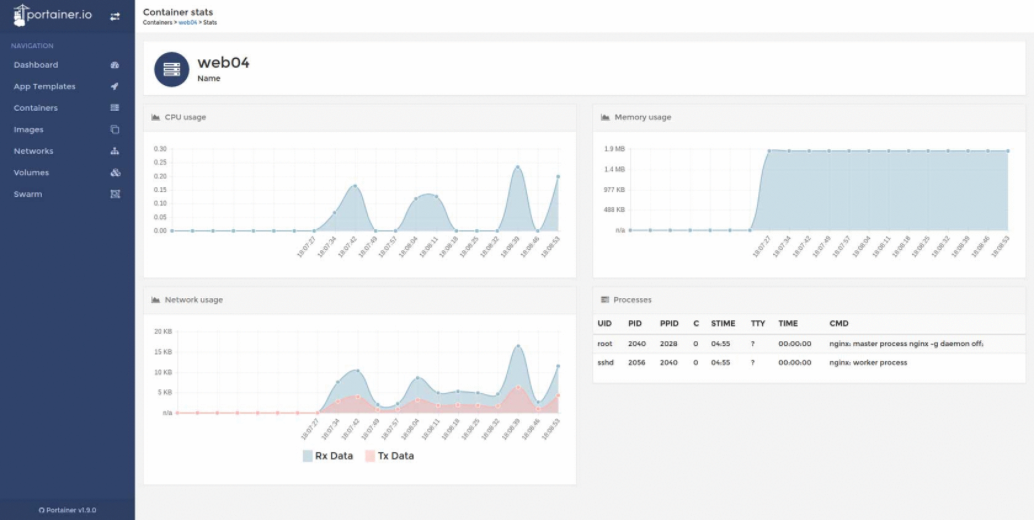
\includegraphics[scale=0.8]{solution-1.png}
	\caption{Сервис Portainer}
\end{figure}
\clearpage